% 第3章第2节：谱与奇异值（谱与特征值、紧自伴算子的谱分解、紧算子的奇异值分解）。

\section{谱与奇异值}
\label{sec:ose-spectrum}

紧算子能被有限秩算子统一逼近，但上一节没有说明应该保留哪些方向、每个方向被放大或压缩多少。有限维中，这个问题由特征值和奇异值回答。本节先用可逆性定义无限维算子的谱，说明它为什么不能只由特征值组成；再在紧自伴条件下建立正交的特征展开；最后对一般紧算子使用输入、输出两组方向，得到奇异值分解及最佳有限秩逼近。

\subsection{谱与特征值}
\label{sec:ose-spectrum-def}

\paragraph{从不可逆性定义谱}
在$n$维空间中，$\bm A-\lambda\bm I$不可逆当且仅当它不是单射，即存在非零向量$\bm v$使$\bm A\bm v=\lambda\bm v$；单射、满射和可逆三者等价，所以“使$\bm A-\lambda\bm I$不可逆的$\lambda$”恰好就是特征值。矩阵的特征值、实对称矩阵的正交对角化与奇异值分解都建立在这一等价关系上，可参考\BookChapterRef{chap:matrix-analysis}{卷一“谱和奇异值”章}。无限维中三者不再等价，必须直接从可逆性出发。

\begin{definition}[谱与预解集]
\label{def:ose-spectrum}
设$H$为复Hilbert空间，$A\in\mathcal B(H)$。若$A-\lambda I$是$H$到$H$的双射，且逆映射$(A-\lambda I)^{-1}$有界，则称$\lambda\in\mathbb C$属于$A$的\term{预解集}（resolvent set），记为$\rho(A)$，并称$(A-\lambda I)^{-1}$为\term{预解算子}（resolvent operator）。预解集的补集$\sigma(A)=\mathbb C\setminus\rho(A)$称为$A$的\term{谱}（spectrum）。若存在非零$u\in H$使$Au=\lambda u$，则称$\lambda$为$A$的\term{特征值}（eigenvalue），$u$为相应的\term{特征向量}（eigenvector）；在函数空间中也常称特征函数。
\end{definition}

由第~\ref{sec:lfo-open-mapping}节的有界逆定理，Banach空间之间的有界线性双射自动有有界逆，所以定义中“逆有界”一项对$A-\lambda I$是全空间双射的情形并不额外增加限制。写出这一项是为了强调：预解参数要求在\emph{整个}$H$上能够稳定地反解$(A-\lambda I)u=g$。特征值使$A-\lambda I$有非零核，当然属于谱；但$A-\lambda I$也可能是单射却不满射，此时只能在像上定义逆映射，这个逆映射还可能没有统一的界。这两种情形都使$\lambda$进入谱，却都不对应非零特征向量。

\paragraph{对角算子的谱}
回到$\ell^2$上的$A(x_n)=(x_n/n)$，逐个检查$\lambda$。若$\lambda=1/k$，则$Ae_k=e_k/k$，所以每个$1/k$都是特征值，特征向量为$e_k$。

再看$\lambda=0$。若$Ax=0$，则每个$x_n/n=0$，所以$A$是单射，$0$不是特征值。但$A$不是满射：第~\ref{sec:lfo-range-kernel}节已经说明，$y=(1/n)\in\ell^2$的唯一形式逆像是常数列$(1,1,\ldots)$，它不平方可和，故$y\notin\operatorname{Ran}A$。即使只在像上考虑逆映射$y\mapsto(ny_n)$，它把单位向量$e_n$送到$ne_n$，范数为$n$，没有统一的界。所以$0\in\sigma(A)$，却不是特征值。

最后取$\lambda$不在集合$S=\{1/n:n\geq1\}\cup\{0\}$中。$S$是闭集（它唯一的聚点$0$已在其中），所以$d=\operatorname{dist}(\lambda,S)>0$。对每个$n$有$|1/n-\lambda|\geq d$，于是方程$(A-\lambda I)x=y$逐坐标解出
\[
  x_n=\frac{y_n}{1/n-\lambda},\qquad \|x\|\leq\frac{1}{d}\|y\| .
\]
这给出全空间上的有界逆，$\lambda\in\rho(A)$。综合三种情形，
\[
  \sigma(A)=\{1/n:n\geq1\}\cup\{0\},\qquad \|(A-\lambda I)^{-1}\|=\frac{1}{\operatorname{dist}(\lambda,\sigma(A))}\quad(\lambda\in\rho(A)).
\]
范数公式中的上界刚刚得到；取$y=e_n$并让$1/n$逼近离$\lambda$最近的谱点，可知上界不能改进。

\begin{figure}[!htb]
  \centering
  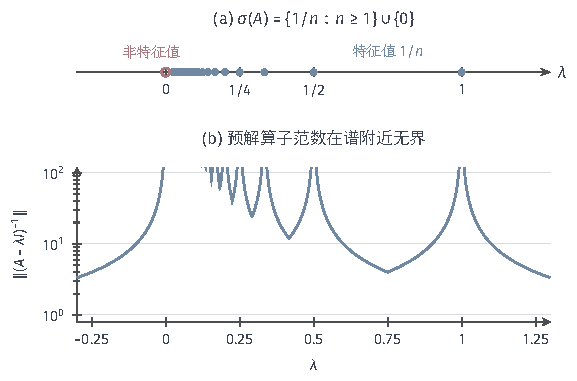
\includegraphics[width=97.8mm]{figures/02-abstract-mathematics/03-function-spaces/tikz/c3-spectrum-resolvent/figure.pdf}
  \caption{$\ell^2$上$A(x_n)=(x_n/n)$的谱。(a) 特征值$1/n$（实心点）向$0$聚集；$0$在谱中但不是特征值（空心点）。(b) 实参数$\lambda$处预解算子的范数$1/\operatorname{dist}(\lambda,\sigma(A))$，纵轴取对数；每个谱点附近范数都无界，在$0$附近这些尖峰挤在一起。}
  \label{fig:ose-spectrum-resolvent}
\end{figure}

图~\ref{fig:ose-spectrum-resolvent}把这三种情形放在一起：特征值是孤立的点，它们聚集到不是特征值的$0$；在任何谱点附近，反解$(A-\lambda I)u=g$的放大倍数都没有上界。三种情形对应三种不同的方向信息：特征值$1/n$对应被精确缩放的方向$e_n$；$0$不对应任何被消去的方向，而是对应一列被压得越来越扁的方向，使像空间稠密却不闭合；远离谱的$\lambda$则让每个方向的缩放倍数$1/n-\lambda$都离零有一段距离。

这一现象对紧算子是普遍的。若$H$无限维而紧算子$A$有有界逆，则$I=A^{-1}A$作为有界算子与紧算子的复合仍是紧算子（有界输入列经$A$后有收敛子列，再经连续的$A^{-1}$仍收敛），与第~\ref{sec:ose-compact-def}小节中单位算子不紧矛盾。所以无限维空间中的紧算子总有$0\in\sigma(A)$，无论$0$是否为特征值。

实Hilbert空间中的算子可以先扩张到复化空间再讨论谱；对下面的自伴算子，特征值都是实数，这样做不会产生新的困难。一般非自伴算子的谱可能含有非实数，其谱分类不在本章展开。

\subsection{紧自伴算子的谱分解}
\label{sec:ose-spectral-theorem}

对角算子的例子中，特征向量$e_n$恰好组成标准正交基，算子就是沿每个基方向乘以一个数。实对称矩阵具有同样的结构：存在由特征向量组成的标准正交基，矩阵在这组基下是实对角矩阵。本小节证明，紧自伴算子在无限维中保留了这一结构：非零特征值至多可数并只能聚集到零，特征方向两两正交，并且与核一起张满整个空间。

\paragraph{紧自伴谱分解的陈述}
自伴算子的定义见第~\ref{sec:lfo-self-adjoint}节：$A\in\mathcal B(H)$满足$A^*=A$，即$\langle v,Au\rangle=\langle Av,u\rangle$对所有$u,v$成立。

\begin{theorem}[紧自伴算子的谱分解]
\label{thm:ose-compact-selfadjoint}
设$H$为实或复Hilbert空间，$A:H\to H$为紧自伴算子。则：
\begin{enumerate}
  \item $A$的特征值都是实数，属于不同特征值的特征向量互相正交；
  \item 每个非零特征值的特征空间有限维；对每个$\delta>0$，满足$|\lambda|\geq\delta$的特征值只有有限个，因此非零特征值至多可数，并且只可能在$0$处聚集；
  \item 存在有限或可数的标准正交序列$(e_j)$及非零实数$\lambda_j$（按重数重复列出，$|\lambda_1|\geq|\lambda_2|\geq\cdots$，序列无限时$\lambda_j\to0$），使$Ae_j=\lambda_je_j$，$(e_j)$的闭张成等于$(\ker A)^\perp$，并且对每个$u\in H$，
  \begin{equation}
    u=u_0+\sum_j\langle e_j,u\rangle e_j,\qquad Au=\sum_j\lambda_j\langle e_j,u\rangle e_j,\qquad u_0\in\ker A,
    \label{eq:ose-spectral-expansion}
  \end{equation}
  两个级数都按$H$的范数收敛。
\end{enumerate}
\end{theorem}

证明的主线是：先说明自伴算子的范数可以由二次型$\langle u,Au\rangle$读出，再用紧性找到使二次型绝对值达到最大的方向，它就是一个特征方向；然后把算子限制到这个方向的正交补上，重复同样的步骤。下面分步完成。

\paragraph{特征值与正交性}
设$Au=\lambda u$，$u\neq0$。由内积对第二变量线性、对第一变量共轭线性，$\langle u,Au\rangle=\lambda\|u\|^2$，$\langle Au,u\rangle=\overline\lambda\|u\|^2$；自伴使两者相等，所以$\lambda=\overline\lambda$为实数。再设$Av=\mu v$，$\mu\neq\lambda$，两者都是实数，于是
\[
  \lambda\langle v,u\rangle=\langle v,Au\rangle=\langle Av,u\rangle=\mu\langle v,u\rangle ,
\]
从而$\langle v,u\rangle=0$。这证明了结论1。

\paragraph{非零特征值的有限性}
设$(e_j)$是一列两两正交的单位特征向量，$Ae_j=\lambda_je_j$且$|\lambda_j|\geq\delta>0$。这种序列可以来自同一个特征空间的标准正交组，也可以来自不同特征值（由结论1自动正交）。对$j\neq k$，
\[
  \|Ae_j-Ae_k\|^2=\|\lambda_je_j-\lambda_ke_k\|^2=|\lambda_j|^2+|\lambda_k|^2\geq2\delta^2 ,
\]
输出列没有柯西子列，与紧性矛盾。所以这种序列只能有限长。取同一特征空间中的标准正交组，即知非零特征空间有限维；取不同特征值的特征向量，即知$|\lambda|\geq\delta$的特征值只有有限个。令$\delta=1,1/2,1/3,\ldots$，非零特征值是可数个有限集合的并，且任何$\delta>0$之外只有有限个，只能在$0$处聚集。这证明了结论2。

\paragraph{二次型给出范数}
设$A$自伴，令$M=\sup_{\|u\|=1}|\langle u,Au\rangle|$。由Cauchy–Schwarz不等式，$|\langle u,Au\rangle|\leq\|A\|$，故$M\leq\|A\|$。反向不等式要从二次型恢复$\|Au\|$。自伴性使$\langle u,Au\rangle=\langle Au,u\rangle=\overline{\langle u,Au\rangle}$为实数，展开可得
\[
  \langle u+v,A(u+v)\rangle-\langle u-v,A(u-v)\rangle=2\langle u,Av\rangle+2\langle v,Au\rangle=4\operatorname{Re}\langle v,Au\rangle ,
\]
其中用到$\langle u,Av\rangle=\langle Au,v\rangle=\overline{\langle v,Au\rangle}$。左边两项各自的绝对值不超过$M\|u\pm v\|^2$，再用平行四边形恒等式$\|u+v\|^2+\|u-v\|^2=2\|u\|^2+2\|v\|^2$，
\[
  4\operatorname{Re}\langle v,Au\rangle\leq M\bigl(\|u+v\|^2+\|u-v\|^2\bigr)=2M\bigl(\|u\|^2+\|v\|^2\bigr).
\]
对单位向量$u$且$Au\neq0$，取$v=Au/\|Au\|$，则$\operatorname{Re}\langle v,Au\rangle=\|Au\|$，上式化为$4\|Au\|\leq4M$。因此$\|A\|\leq M$，两者相等。

\paragraph{紧性给出极值方向}
现设$A\neq0$紧自伴。取单位向量$u_n$使$|\langle u_n,Au_n\rangle|\to\|A\|$。这些二次型都是实数，绝对值趋于$\|A\|>0$，可以抽出子列使它们的符号一致，于是沿该子列$\langle u_n,Au_n\rangle\to\lambda$，其中$\lambda=\|A\|$或$\lambda=-\|A\|$。这里不能预先假定$\lambda$为正：自伴算子的二次型可以取负值，绝对值最大的特征值可能是负的。展开
\[
  \|Au_n-\lambda u_n\|^2=\|Au_n\|^2-2\lambda\langle u_n,Au_n\rangle+\lambda^2\leq2\lambda^2-2\lambda\langle u_n,Au_n\rangle\to0 ,
\]
其中用到$\|Au_n\|\leq\|A\|=|\lambda|$。由紧性，可再抽子列使$Au_n\to w$。于是$\lambda u_n=Au_n-(Au_n-\lambda u_n)\to w$，即$u_n\to e=w/\lambda$，且$\|e\|=1$。由$A$连续，$Ae=\lim Au_n=w=\lambda e$。所以$\pm\|A\|$中至少有一个是特征值，且对应单位特征向量$e$。

\paragraph{逐步分解与核}
记$e_1=e$，$\lambda_1=\lambda$。正交补$H_2=\{e_1\}^\perp$在$A$下不变：若$\langle e_1,v\rangle=0$，则$\langle e_1,Av\rangle=\langle Ae_1,v\rangle=\lambda_1\langle e_1,v\rangle=0$。$A$在$H_2$上的限制仍是紧自伴算子，范数不超过$\|A\|$。若这个限制为零，过程停止；否则对它重复上一段，得到$e_2\perp e_1$及$|\lambda_2|=\|A|_{H_2}\|\leq|\lambda_1|$。依此类推，在$H_k=\{e_1,\ldots,e_{k-1}\}^\perp$上取$e_k$，得到$|\lambda_1|\geq|\lambda_2|\geq\cdots$。若过程不停止，由结论2，$\lambda_k\to0$。

令$M$为$(e_j)$的闭张成。$M^\perp$含于每个$H_k$，所以$A$在$M^\perp$上的限制的范数不超过每个$|\lambda_k|$；过程无限时它趋于零，有限时按停止条件本身为零。因此$A$在$M^\perp$上恒为零，$M^\perp\subseteq\ker A$。反过来，若$Au=0$，则对每个$j$，
\[
  \langle e_j,u\rangle=\frac{1}{\lambda_j}\langle Ae_j,u\rangle=\frac{1}{\lambda_j}\langle e_j,Au\rangle=0 ,
\]
所以$\ker A\subseteq M^\perp$。二者相等，$M=(M^\perp)^\perp=(\ker A)^\perp$。这同时说明每个非零特征值都已出现在$(\lambda_j)$中：属于非零特征值$\mu$的特征向量与$\ker A$正交，因而落在$M$中；若$\mu$不等于任何$\lambda_j$，它就与所有$e_j$正交，只能为零。

\paragraph{展开式}
由第~\ref{sec:fs-orthogonal-expansion}节，$u$在闭子空间$M$上的正交投影为$\sum_j\langle e_j,u\rangle e_j$，级数按范数收敛；余项$u_0$属于$M^\perp=\ker A$。把$A$作用于投影的部分和，由连续性得到$Au=\sum_j\lambda_j\langle e_j,u\rangle e_j$。这就是式~\eqref{eq:ose-spectral-expansion}，证毕。

\paragraph{贯穿例子中的谱分解}
在$L^2([-1,1],\mu)$上，$d\mu=dz/2$，核$K(x,z)=1+xz$给出$(Tf)(x)=\int f\,d\mu+x\int zf\,d\mu$。由$\int1\,d\mu=1$与$\int z^2\,d\mu=\frac12\int_{-1}^{1}z^2\,dz=\frac13$，
\[
  T1=1,\qquad Tx=x\int z^2\,d\mu=\tfrac13x .
\]
单位化得$e_1=1$、$e_2=\sqrt3\,x$（因为$\int3x^2\,d\mu=1$），特征值$\lambda_1=1$、$\lambda_2=1/3$。式~\eqref{eq:ose-spectral-expansion}化为
\[
  Tf=\langle e_1,f\rangle e_1+\tfrac13\langle e_2,f\rangle e_2 ,
\]
与$1,x$都正交的函数组成$\ker T$，它是无限维的。第~\ref{sec:ose-kernels}小节将在积分核的语言下再看这个例子。

把核换成$1-6xz$，常数方向不变，线性方向变为$T x=-6x\int z^2\,d\mu=-2x$，特征值$-2$的绝对值最大。图~\ref{fig:ose-spectral-stretch}(b)在$e_1,e_2$的系数平面上画出单位圆的像：沿$e_1$方向不变，沿$e_2$方向拉长两倍并翻转，点$p$被送到$e_2$坐标反号的$Tp$。若只寻找正的最大特征值，就会漏掉这个主导方向。图~\ref{fig:ose-spectral-stretch}(a)则显示$\ell^2$对角算子的情形：$u$的每个系数$\langle e_j,u\rangle$被乘以$\lambda_j=1/j$，后面的方向被压得更小。

\begin{figure}[!htb]
  \centering
  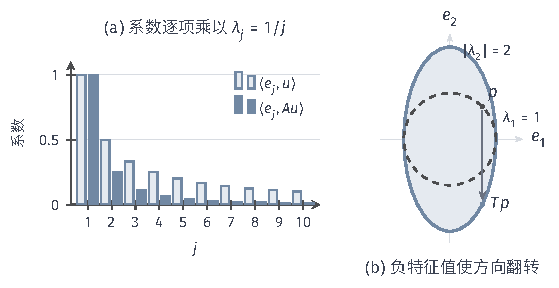
\includegraphics[width=94.6mm]{figures/02-abstract-mathematics/03-function-spaces/tikz/c3-spectral-stretch/figure.pdf}
  \caption{紧自伴算子沿特征方向逐个伸缩。(a) $\ell^2$上$A=\operatorname{diag}(1/j)$，浅色条为$u$的系数$\langle e_j,u\rangle=1/j$，深色条为$Au$的系数$1/j^2$。(b) $L^2([-1,1],dz/2)$上核$1-6xz$的积分算子，在$e_1=1$、$e_2=\sqrt3x$的系数平面上把虚线单位圆映为实线椭圆：$e_1$方向乘$1$，$e_2$方向乘$-2$。与$1,x$正交的方向全部被映为零，图中未画出。}
  \label{fig:ose-spectral-stretch}
\end{figure}

\paragraph{展开的收敛方式}
式~\eqref{eq:ose-spectral-expansion}中的级数按Hilbert空间的范数收敛。对$L^2(\mu)$中的函数，这意味着平方积分误差趋于零，并不意味着在每个点或一致地收敛；$L^2$的元素本来就是几乎处处等价类，单独谈某一点的值没有意义。若要把特征展开写成核函数$K(x,z)=\sum_j\lambda_je_j(x)\overline{e_j(z)}$的逐点甚至一致收敛的级数，需要核连续、半正定等额外条件，这是第~\ref{sec:rkhs-mercer}节Mercer定理讨论的内容。

\subsection{紧算子的奇异值分解}
\label{sec:ose-svd}

非自伴算子不一定有足够多的特征向量，输入与输出甚至可以位于不同的空间。有限维中，矩阵的奇异值分解用输入、输出各一组标准正交方向解决这个问题。对紧算子，同样的构造可以通过正紧自伴算子$A^*A$完成。

\paragraph{从$A^*A$构造两组方向}
设$H_1,H_2$为Hilbert空间，$A:H_1\to H_2$为紧算子。$A^*A:H_1\to H_1$是紧算子：有界输入列经$A$后有收敛子列，再经连续的$A^*$仍收敛。它也是自伴的，且
\[
  \langle x,A^*Ax\rangle=\langle Ax,Ax\rangle=\|Ax\|^2\geq0 ,
\]
所以它的特征值都非负，并且$A^*Ax=0$当且仅当$Ax=0$，即$\ker(A^*A)=\ker A$。

对$A^*A$应用定理~\ref{thm:ose-compact-selfadjoint}，得到标准正交的特征向量$v_j$与正特征值$s_j$，按递减顺序排列。令$\sigma_j=\sqrt{s_j}$，再令$u_j=Av_j/\sigma_j$。这组输出方向也是标准正交的：
\[
  \langle u_j,u_k\rangle=\frac{\langle Av_j,Av_k\rangle}{\sigma_j\sigma_k}=\frac{\langle v_j,A^*Av_k\rangle}{\sigma_j\sigma_k}=\frac{\sigma_k^2\langle v_j,v_k\rangle}{\sigma_j\sigma_k}=\delta_{j,k} .
\]
此外$A^*u_j=A^*Av_j/\sigma_j=\sigma_jv_j$，所以$A$把$v_j$送到$\sigma_ju_j$，$A^*$把$u_j$送回$\sigma_jv_j$。

\begin{theorem}[紧算子的奇异值分解]
\label{thm:ose-svd}
设$A:H_1\to H_2$为紧算子，$\sigma_1\geq\sigma_2\geq\cdots>0$及标准正交序列$(v_j)\subset H_1$、$(u_j)\subset H_2$如上构造。则对每个$x\in H_1$、$y\in H_2$，
\begin{equation}
  Ax=\sum_j\sigma_j\langle v_j,x\rangle u_j,\qquad A^*y=\sum_j\sigma_j\langle u_j,y\rangle v_j ,
  \label{eq:ose-svd}
\end{equation}
级数按范数收敛。$(v_j)$的闭张成为$(\ker A)^\perp$，$(u_j)$的闭张成为$\overline{\operatorname{Ran}A}=(\ker A^*)^\perp$。序列无限时$\sigma_j\to0$。
\end{theorem}

\begin{proof}
由定理~\ref{thm:ose-compact-selfadjoint}，$(v_j)$的闭张成为$(\ker A^*A)^\perp=(\ker A)^\perp$，任意$x$可写成$x=x_0+\sum_j\langle v_j,x\rangle v_j$，$x_0\in\ker A$。把$A$作用于部分和并取极限，得$Ax=\sum_j\langle v_j,x\rangle Av_j=\sum_j\sigma_j\langle v_j,x\rangle u_j$。由这一展开，每个$Ax$都落在$(u_j)$的闭张成中；反之每个$u_j=A(v_j/\sigma_j)$属于$\operatorname{Ran}A$。所以$(u_j)$的闭张成等于$\overline{\operatorname{Ran}A}$，再由第~\ref{sec:lfo-range-kernel}节得它等于$(\ker A^*)^\perp$。关于$A^*$的展开，对任意$x$有
\[
  \langle x,A^*y\rangle=\langle Ax,y\rangle=\sum_j\sigma_j\overline{\langle v_j,x\rangle}\langle u_j,y\rangle=\Bigl\langle x,\sum_j\sigma_j\langle u_j,y\rangle v_j\Bigr\rangle ,
\]
右端级数因系数平方可和而收敛，两边对所有$x$相等，故展开成立。$\sigma_j\to0$来自$s_j\to0$。
\end{proof}

数$\sigma_j$称为$A$的\term{奇异值}（singular value），$v_j$与$u_j$分别称为\term{右奇异向量}（right singular vector）与\term{左奇异向量}（left singular vector）。展开式~\eqref{eq:ose-svd}说明$A$的作用分三步：读出输入在$v_j$方向上的系数，乘以$\sigma_j$，再放到输出方向$u_j$上。输入中的$\ker A$完全看不见；输出中的$\ker A^*$则是永远到达不了的方向。两组方向一般属于不同的空间，即使$H_1=H_2$，$u_j$也未必等于$v_j$；只有正自伴算子才使两组方向重合、奇异值等于特征值。

\begin{example}[积分算子的奇异值分解]
\label{ex:ose-volterra-svd}
在$L^2(0,1)$上（Lebesgue测度），令$(Vf)(x)=\int_0^xf(t)\,dt$。它是核$\mathbf 1_{\{t<x\}}$的积分算子；这个核在$[0,1]^2$上平方可积，第~\ref{sec:ose-hilbert-schmidt}小节将证明这样的积分算子是紧算子，这里先承认这一点。由Fubini定理交换积分次序，伴随为$(V^*g)(t)=\int_t^1g(x)\,dx$，于是
\[
  (V^*Vf)(t)=\int_t^1\Bigl(\int_0^xf(s)\,ds\Bigr)dx .
\]

设$V^*Vf=sf$，$s>0$。右端是连续函数，所以$f=s^{-1}V^*Vf$连续；于是$Vf$连续可微，$V^*Vf$二次连续可微，$f$也二次连续可微。对$t$求导两次得$(V^*Vf)'=-Vf$、$(V^*Vf)''=-f$，因此$sf''=-f$；又由表达式直接读出$(V^*Vf)'(0)=0$、$(V^*Vf)(1)=0$，故$f'(0)=0$、$f(1)=0$。满足这些条件的非零解为$f(t)=c\cos(\omega t)$，其中$\omega=s^{-1/2}$且$\cos\omega=0$，即$\omega_k=(k-\tfrac12)\pi$，$k=1,2,\ldots$。

$V$是单射：若$\int_0^xf=0$对所有$x$成立，则$E\mapsto\int_Ef^+$与$E\mapsto\int_Ef^-$在所有区间上相等，由定理~\ref{thm:measure-pi-lambda-uniqueness}在全部Borel集上相等，取$E=\{f>0\}$即知$f\leq0$几乎处处，同理$f\geq0$几乎处处。于是$\ker V^*V=\ker V=\{0\}$，由定理~\ref{thm:ose-compact-selfadjoint}，$V^*V$的特征向量张满整个$L^2(0,1)$。由此得到
\[
  \sigma_k=\frac{1}{(k-\frac12)\pi}=\frac{2}{(2k-1)\pi},\qquad
  \begin{aligned}
    v_k(t)&=\sqrt2\cos\bigl((k-\tfrac12)\pi t\bigr),\\
    u_k(x)&=\sqrt2\sin\bigl((k-\tfrac12)\pi x\bigr),
  \end{aligned}
\]
其中$u_k=Vv_k/\sigma_k$可直接积分验证。前几个奇异值约为$0.637$、$0.212$、$0.127$、$0.091$，按$1/k$的速度衰减。
\end{example}

\paragraph{截断奇异值与最佳有限秩逼近}
奇异值分解直接给出有限秩逼近：只保留前$m$项，
\[
  A_mx=\sum_{j\leq m}\sigma_j\langle v_j,x\rangle u_j .
\]
下面的定理说明这个截断的误差恰为下一个奇异值，并且没有任何秩不超过$m$的算子做得更好。若正奇异值只有有限个，约定用尽之后的$\sigma_j=0$。

\begin{theorem}[截断奇异值分解的最优性]
\label{thm:ose-svd-truncation}
在定理~\ref{thm:ose-svd}的条件下，$\|A-A_m\|=\sigma_{m+1}$；对每个秩不超过$m$的有界算子$F:H_1\to H_2$，都有$\|A-F\|\geq\sigma_{m+1}$。
\end{theorem}

\begin{proof}
第一步，计算截断误差。由式~\eqref{eq:ose-svd}及$(u_j)$的正交性，
\[
  \|(A-A_m)x\|^2=\sum_{j>m}\sigma_j^2|\langle v_j,x\rangle|^2\leq\sigma_{m+1}^2\sum_{j>m}|\langle v_j,x\rangle|^2\leq\sigma_{m+1}^2\|x\|^2 ,
\]
其中最后一步是Bessel不等式。取$x=v_{m+1}$时等号成立（若$\sigma_{m+1}=0$，结论已由上式得到），所以$\|A-A_m\|=\sigma_{m+1}$。

第二步，证明下界。不妨设$\sigma_{m+1}>0$。令$W=\operatorname{span}\{v_1,\ldots,v_{m+1}\}$，它是$m+1$维的。$F$在$W$上的限制把$W$映入维数不超过$m$的$\operatorname{Ran}F$，由线性代数的维数公式，存在单位向量$x\in W$使$Fx=0$。写$x=\sum_{j\leq m+1}c_jv_j$，$\sum_j|c_j|^2=1$，则
\[
  \|(A-F)x\|^2=\|Ax\|^2=\sum_{j\leq m+1}\sigma_j^2|c_j|^2\geq\sigma_{m+1}^2 .
\]
因此$\|A-F\|\geq\sigma_{m+1}$。
\end{proof}

\begin{figure}[!htb]
  \centering
  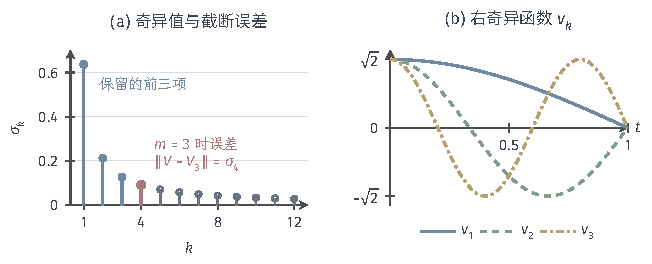
\includegraphics[width=110.3mm]{figures/02-abstract-mathematics/03-function-spaces/tikz/c3-svd-decay/figure.pdf}
  \caption{积分算子$(Vf)(x)=\int_0^xf$在$L^2(0,1)$上的奇异值分解。(a) 奇异值$\sigma_k=2/((2k-1)\pi)$；保留前三项（蓝色）时，算子范数误差等于第四个奇异值$\sigma_4\approx0.091$（红色），后面的奇异值（空心）全部被舍去。(b) 前三个右奇异函数$v_k(t)=\sqrt2\cos((k-\frac12)\pi t)$，序号越大振荡越快。}
  \label{fig:ose-svd-decay}
\end{figure}

图~\ref{fig:ose-svd-decay}在积分算子$V$上展示这一结论。保留前三项时误差为$\sigma_4\approx0.091$；奇异值衰减越快，同样秩的截断误差越小。右图显示，奇异值越小的方向振荡越快：$V$是积分，它把快速振荡的输入平均掉，输出的幅度只剩$1/\omega_k$倍。对比$\ell^2$上的$A(x_n)=(x_n/n)$，它是正自伴算子，奇异值就是特征值$1/n$，左右奇异向量都是$e_n$，例~\ref{ex:ose-diagonal-finite-rank}中的截断正是截断奇异值分解。

小奇异值对正向逼近是好消息：它们可以被舍去而误差很小。对反向求解却是坏消息：要从输出恢复输入，必须把这些方向上的系数除以$\sigma_j$。这一障碍留到第~\ref{sec:ose-first-kind}小节处理。
